\documentclass[12pt]{extarticle}
\usepackage{tempora}
\usepackage[T1, T2A]{fontenc}
\usepackage[utf8]{inputenc}
\usepackage[english, ukrainian]{babel}
\usepackage{geometry}
\usepackage{graphicx}
\usepackage{multirow}
\usepackage{multicol}
\usepackage{float}
\usepackage{indentfirst}
\graphicspath{{/home/artem/Pictures}}
\geometry
{
    a4paper,
    left=30mm,
    top=15mm,
    right=20mm,
    bottom=15mm,
}

\begin{document}
\begin{titlepage}
    \begin{center}
        \textbf{\normalsize{\MakeUppercase{
            Міністерство Освіти і науки України
            Національний університет "Львівська політехніка"
        }}}

        \begin{flushright}
        \textbf{ІКНІ}\\
        Кафедра \textbf{ПЗ}
        \end{flushright}
        \vspace{15mm}

        \includegraphics[width=0.4\textwidth]{lpnu_logo.png}

        \vspace*{\fill}

        \textbf{\normalsize{\MakeUppercase{Звіт}}}
            
        До лабораторної роботи №13

        \textbf{на тему:} “ДОСЛІДЖЕННЯ ПРОТОКОЛІВ
        SMTP І POP3”

        \textbf{з дисципліни:} “Організація комп'ютерних мереж”
            
        \vspace*{\fill}

        \begin{flushright}

            \textbf{Лектор:}\\
            доцент кафедри ПЗ\\
            Крук О.Г.\\
            \vspace{12pt}

            \textbf{Виконав:}\\
            студент групи ПЗ-24\\
            Губик А. С.\\
            \vspace{12pt}

            \textbf{Прийняв:}\\
            доцент кафедри ПЗ\\
            Задорожний І. М.\\
        \vspace{12pt}
        \end{flushright}

        Львів -- 2023
            
            
    \end{center}
\end{titlepage}

\textbf{Тема роботи:} ДОСЛІДЖЕННЯ ПРОТОКОЛІВ
SMTP І POP3
\vspace{12pt}

\textbf{Мета роботи:} Ознайомитися зі службою електронної пошти та основними
командами протоколів SMTP і POP3 і навчитися користуватися утилітою telnet
для зв’язку з серверами вхідної та вихідної пошти.
\subsection*{Теоретичні відомості}
Електронна пошта є популярним засобом комп’ютерного спілкування –
нею користуються щонайменше 50 мільйонів осіб по всьому світу (при цьому
трафік електронної пошти – це усього декілька відсотків мережевого трафіка).
Електронна пошта передбачає взаємодію поштового сервера та поштового
клієнта.
Поштовий сервер зазвичай встановлений у провайдера або в локальній
мережі компанії адресата.
Поштовий клієнт – це програма, за допомогою якої користувач приймає
або відправляє пошту. Існує цілий ряд поштових клієнтів (зокрема, MS Outlook
і The Bat), і всі вони працюють за однаковим принципом.
Поштовий клієнт в літературі часто називають MUA (Mail User Agent,
користувацький поштовий агент), а поштовий сервер – MSA (Mail Submission
Agent, агент передачі електронної пошти).
Для відправлення пошти використовуються один протокол (SMTP), а для
прийому – інші, наприклад, POP3 або IMAP. Надалі вживатимемо назви
SMTP-сервер і POP3-сервер.
Відправлення повідомлення виглядає так.
1. Поштовий клієнт зв’язується з поштовим сервером (через визначений
порт), передаючи йому адресу відправника та одержувача та текст
повідомлення.
Адреса відправника (чи одержувача), e-mail, електронна поштова
скринька, адреса електронної пошти – це ідентифікатор, який однозначно
визначає місце на поштовому сервері (поштову скриньку), де зберігається
кореспонденція користувача.
Адреса електронної пошти визначена у RFC 2822. Вона складається з двох
частин, розділених символом @. Ліва частина адреси (до символу @) означає
ім’я поштової скриньки, а права – доменне ім’я поштового сервера, на якому
ця скринька розміщена.
2. SMTP сервер відправника виділяє з адреси одержувача ім’я поштової
скриньки (назвемо його username) та домене ім’я поштового сервера
одержувача.
SMTP-сервер відправника звертається до DNS-сервера для того, щоб
дізнатися IP-адресу поштового сервера одержувача за його доменним іменем.
\break
\subsection*{Хід роботи}

\begin{figure}[H]
    \centering
    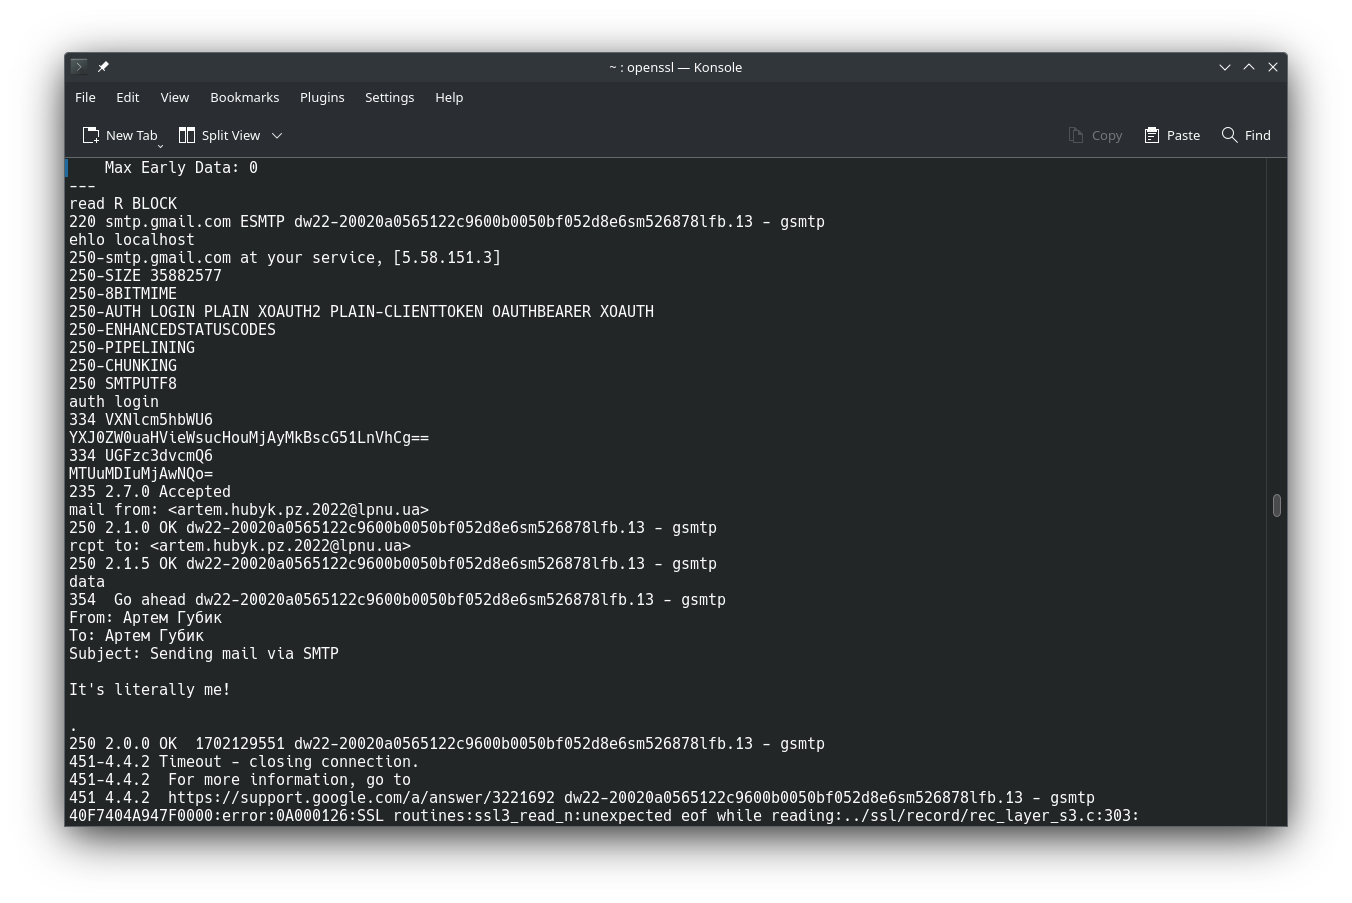
\includegraphics[width=0.90\textwidth]{me}
    \caption{}
\end{figure}



\begin{figure}[H]
    \centering
    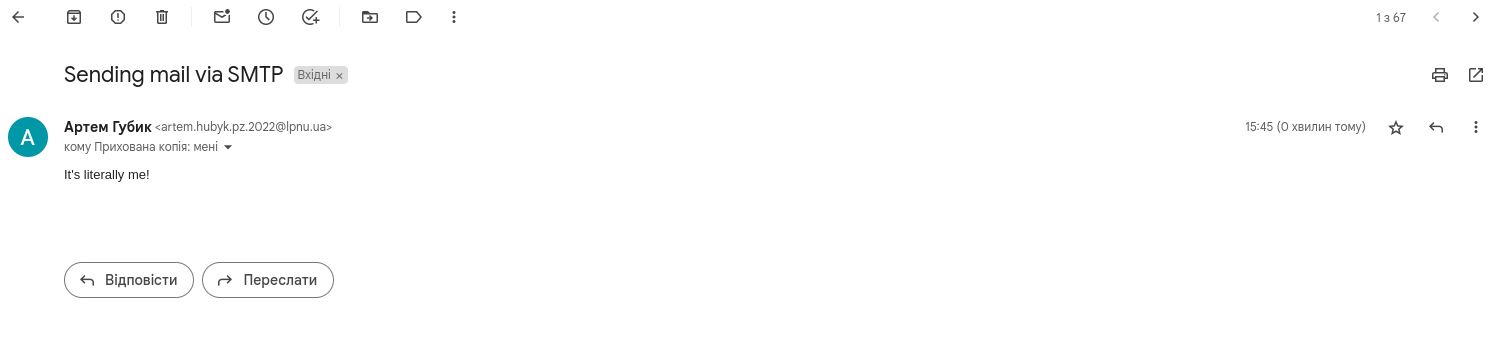
\includegraphics[width=0.90\textwidth]{web}
    \caption{}
\end{figure}

\begin{figure}[H]
    \centering
    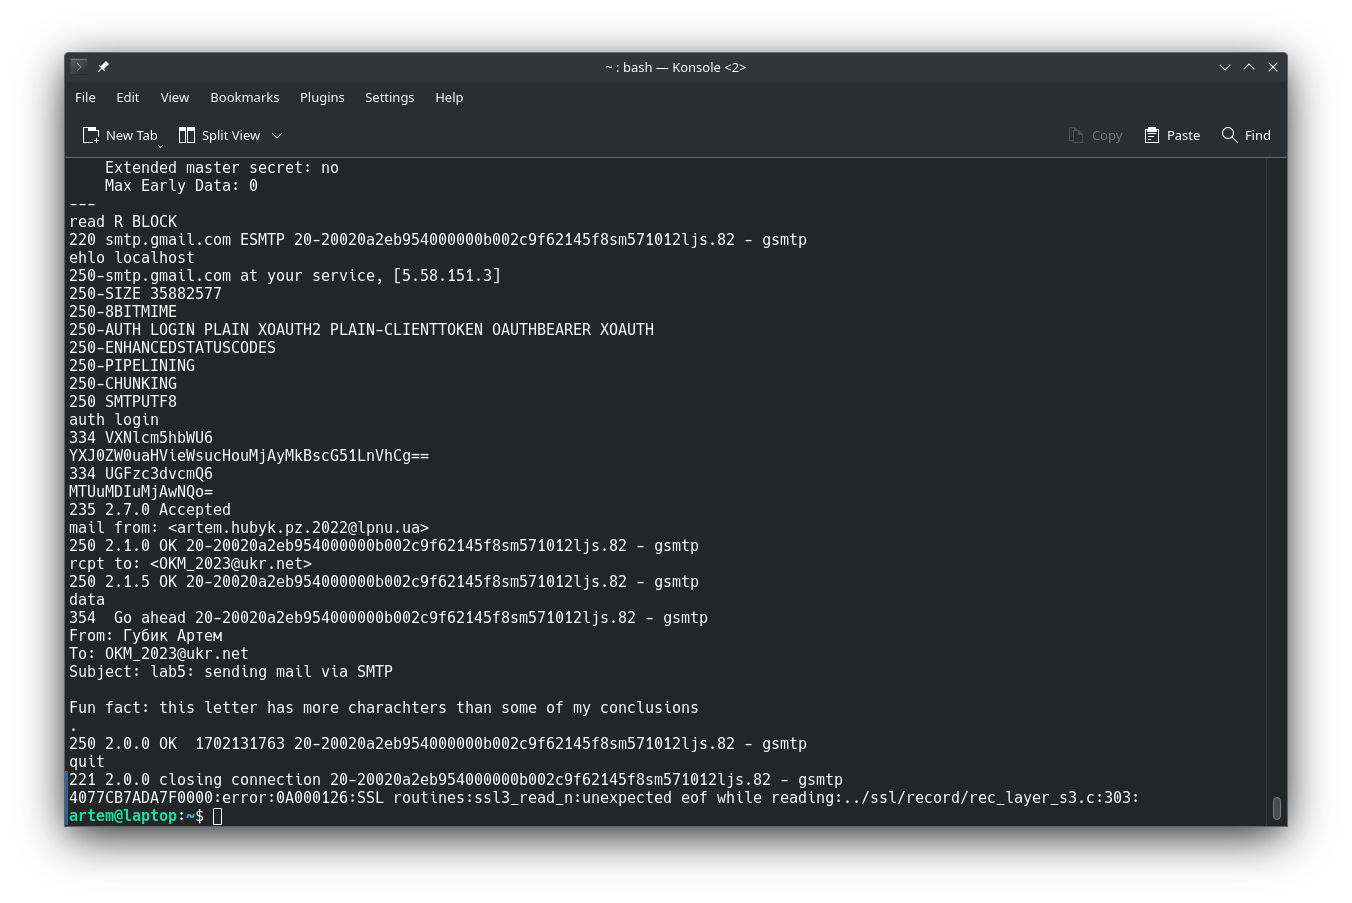
\includegraphics[width=0.90\textwidth]{Screenshot_20231209_162401}
    \caption{}
\end{figure}

\begin{figure}[H]
    \centering
    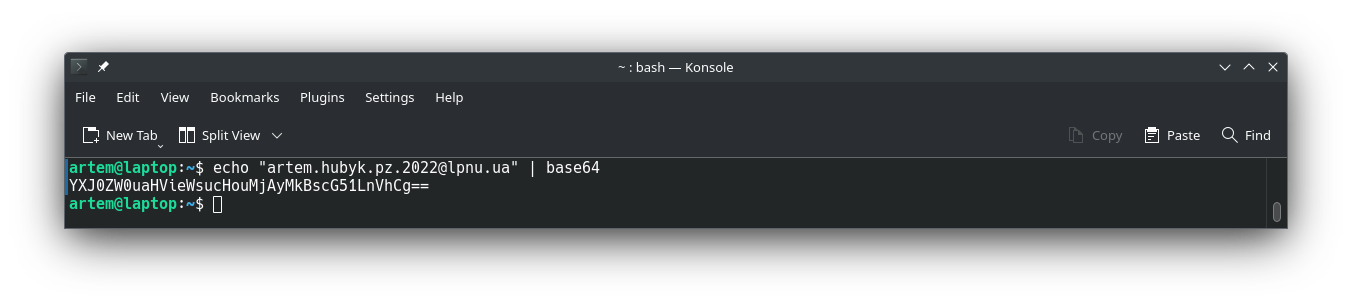
\includegraphics[width=0.90\textwidth]{base64}
    \caption{}
\end{figure}

\begin{figure}[H]
    \centering
    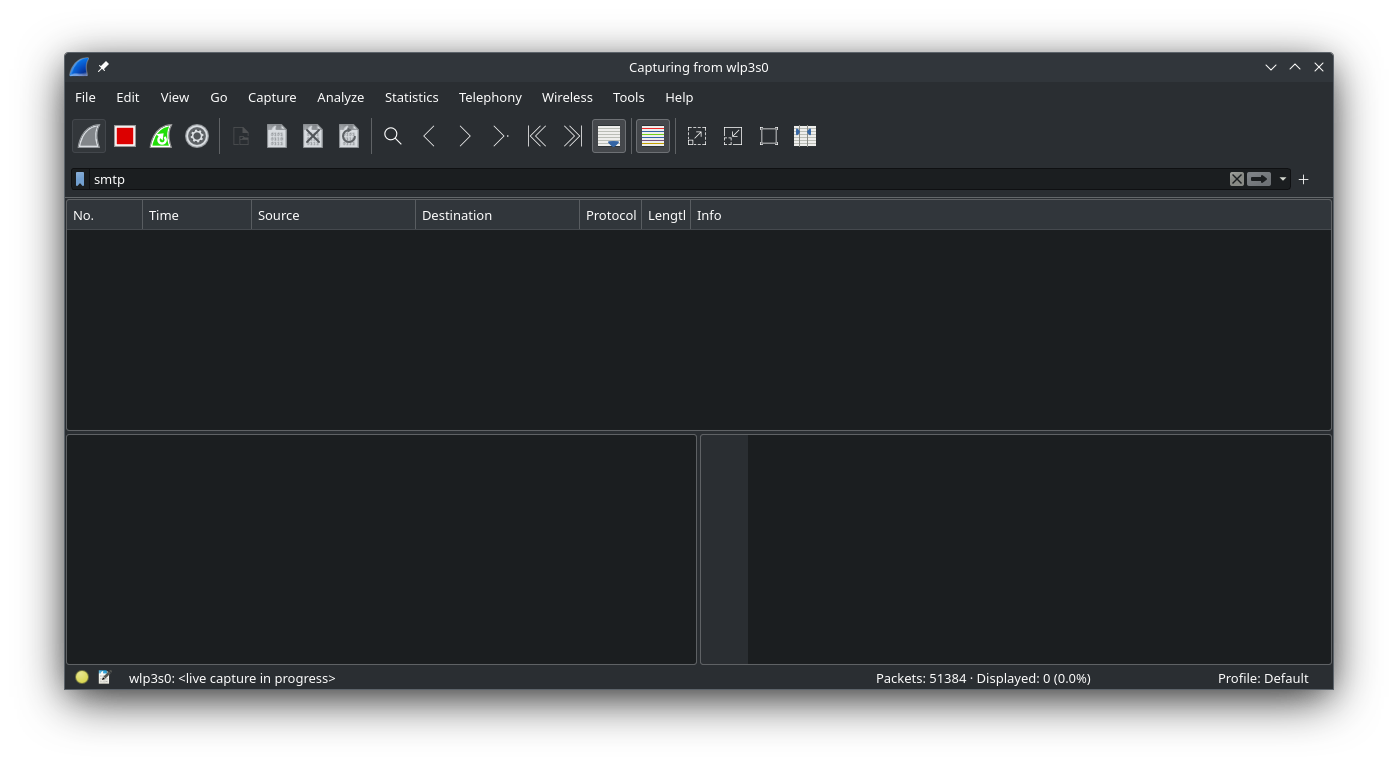
\includegraphics[width=0.90\textwidth]{Screenshot_20231209_162511}
    \caption{}
\end{figure}

\begin{figure}[H]
    \centering
    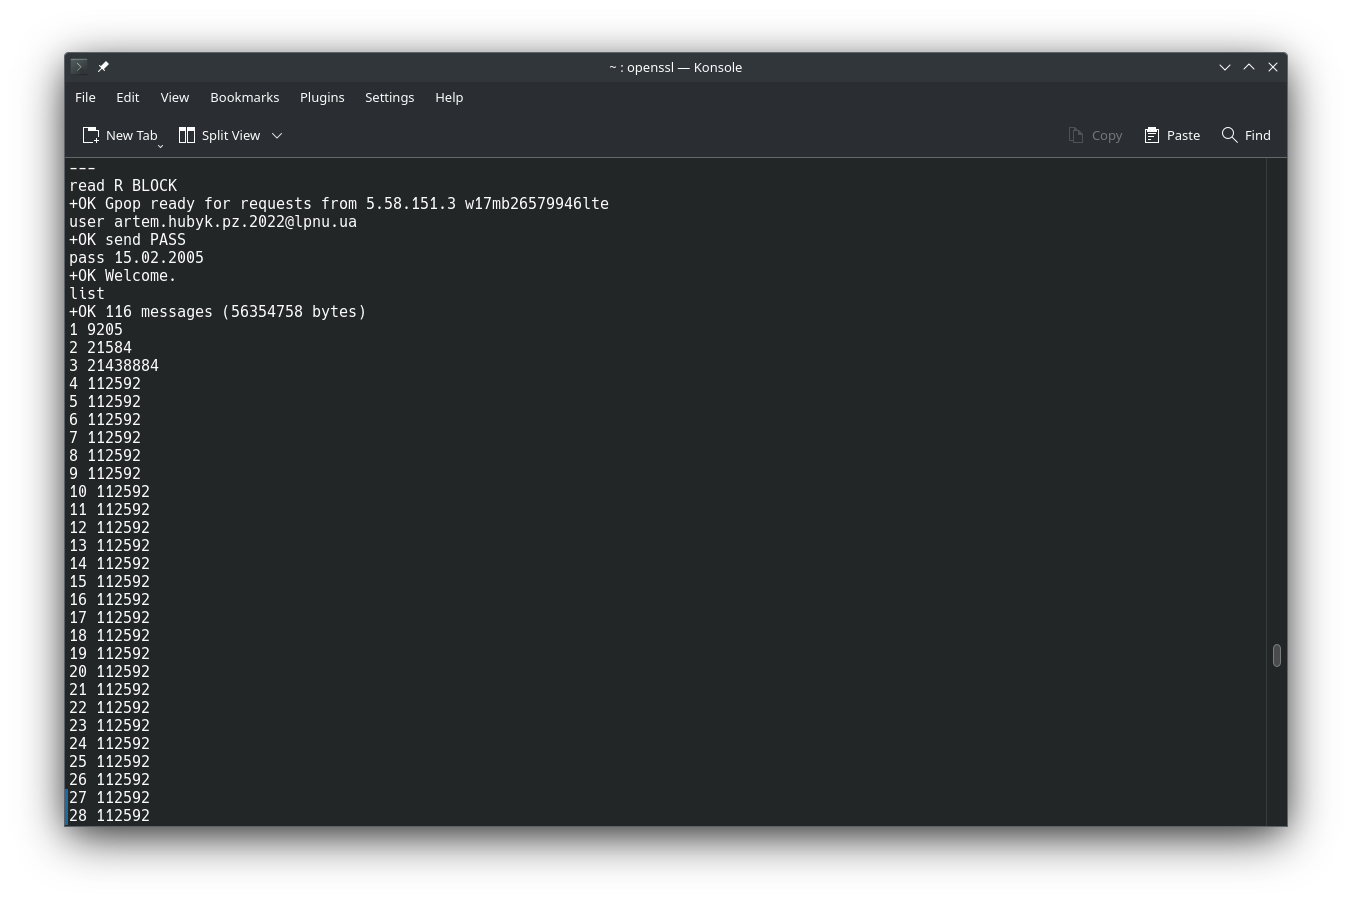
\includegraphics[width=0.90\textwidth]{pop3}
    \caption{}
\end{figure}
\begin{figure}[H]
    \centering
    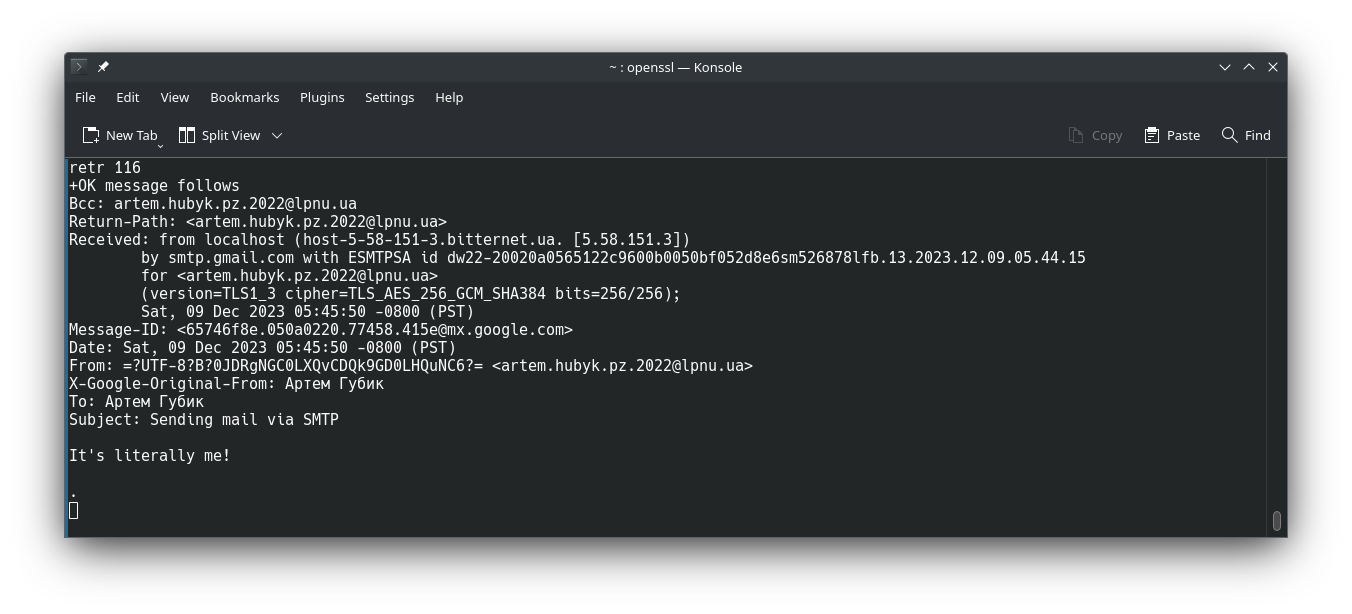
\includegraphics[width=0.90\textwidth]{pop32}
    \caption{}
\end{figure}
\begin{figure}[H]
    \centering
    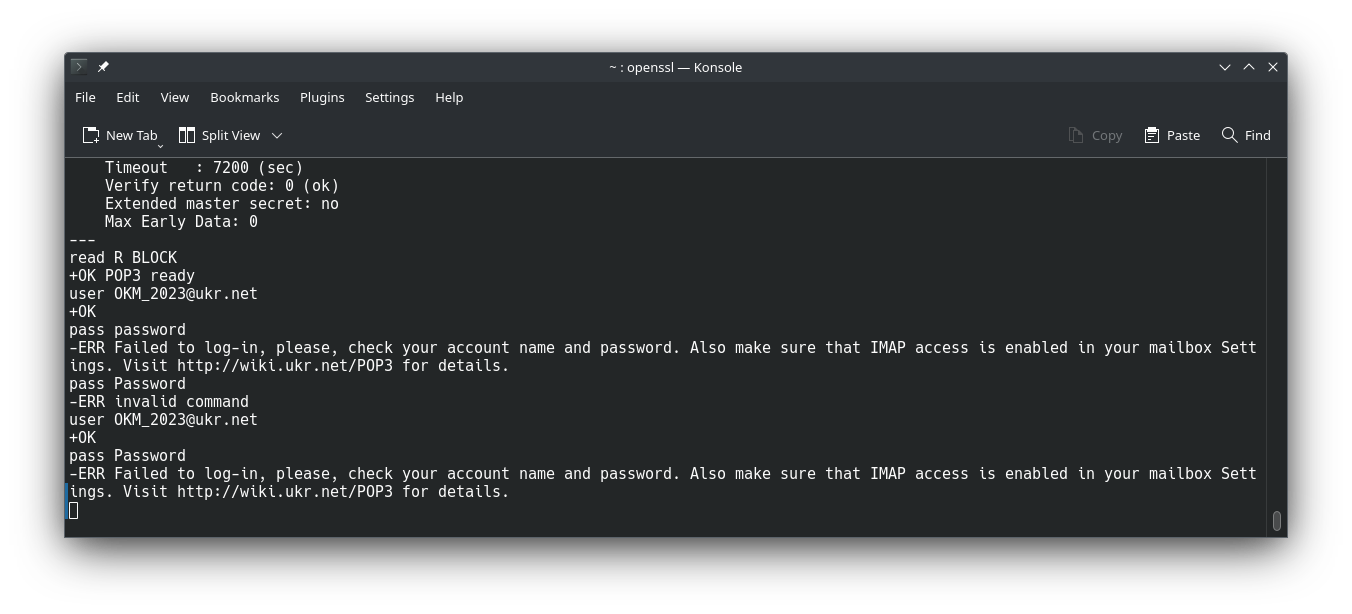
\includegraphics[width=0.90\textwidth]{fail}
    \caption{}
\end{figure}


\subsection*{Висновок} 
Я навчився користуватися OpenSSL, SMTP, POP3 i IMAP. 
\end{document}